%
% Main document
% ===========================================================================
% This is part of the document "Project documentation template".
% Authors: brd3, kaa1
%

%---------------------------------------------------------------------------
\documentclass[
	a4paper,					% paper format
	10pt,							% fontsize
	twoside,					% double-sided
	openright,				% begin new chapter on right side
	notitlepage,			% use no standard title page
	parskip=half,			% set paragraph skip to half of a line
]{scrreprt}					% KOMA-script report
%---------------------------------------------------------------------------

\raggedbottom
\KOMAoptions{cleardoublepage=plain}			% Add header and footer on blank pages


% Load Standard Packages:
%---------------------------------------------------------------------------
\usepackage[standard-baselineskips]{cmbright}

\usepackage[ngerman]{babel}										% german hyphenation
\usepackage[utf8]{inputenc}  							
\usepackage[T1]{fontenc}											% hyphenation of words with ä,ö and ü
\usepackage{textcomp}													% additional symbols
\usepackage{ae}																% better resolution of Type1-Fonts 
\usepackage{fancyhdr}													% simple manipulation of header and footer 
\usepackage{etoolbox}													% color manipulation of header and footer
\usepackage{graphicx}                      		% integration of images
\usepackage{float}														% floating objects
\usepackage{caption}													% for captions of figures and tables
\usepackage{booktabs}													% package for nicer tables
\usepackage{tocvsec2}													% provides means of controlling the sectional numbering
%---------------------------------------------------------------------------

% Load Math Packages
%---------------------------------------------------------------------------
\usepackage{amsmath}                    	   	% various features to facilitate writing math formulas
\usepackage{amsthm}                       	 	% enhanced version of latex's newtheorem
\usepackage{amsfonts}                      		% set of miscellaneous TeX fonts that augment the standard CM
\usepackage{amssymb}													% mathematical special characters
\usepackage{exscale}													% mathematical size corresponds to textsize
%---------------------------------------------------------------------------

% Package to facilitate placement of boxes at absolute positions
%---------------------------------------------------------------------------
\usepackage[absolute]{textpos}
\setlength{\TPHorizModule}{1mm}
\setlength{\TPVertModule}{1mm}
%---------------------------------------------------------------------------					
			
% Definition of Colors
%---------------------------------------------------------------------------
\RequirePackage{color}                          % Color (not xcolor!)
\definecolor{linkblue}{rgb}{0,0,0.8}            % Standard
\definecolor{darkblue}{rgb}{0,0.08,0.45}        % Dark blue
\definecolor{bfhgrey}{rgb}{0.41,0.49,0.57}      % BFH grey
%\definecolor{linkcolor}{rgb}{0,0,0.8}     			% Blue for the web- and cd-version!
\definecolor{linkcolor}{rgb}{0,0,0}        			% Black for the print-version!
%---------------------------------------------------------------------------

% Hyperref Package (Create links in a pdf)
%---------------------------------------------------------------------------
\usepackage[
	pdftex,ngerman,bookmarks,plainpages=false,pdfpagelabels,
	backref = {false},										% No index backreference
	colorlinks = {true},                  % Color links in a PDF
	hypertexnames = {true},               % no failures "same page(i)"
	bookmarksopen = {true},               % opens the bar on the left side
	bookmarksopenlevel = {0},             % depth of opened bookmarks
	pdftitle = {Dokumentation - MindMap},	   	% PDF-property
	pdfauthor = {brd3},        					  % PDF-property
	pdfsubject = {LaTeX Template},        % PDF-property
	linkcolor = {linkcolor},              % Color of Links
	citecolor = {linkcolor},              % Color of Cite-Links
	urlcolor = {linkcolor},               % Color of URLs
]{hyperref}
%---------------------------------------------------------------------------

% Set up page dimension
%---------------------------------------------------------------------------
\usepackage{geometry}
\geometry{
	a4paper,
	left=28mm,
	right=15mm,
	top=30mm,
	headheight=20mm,
	headsep=10mm,
	textheight=242mm,
	footskip=15mm
}
%---------------------------------------------------------------------------

% Makeindex Package
%---------------------------------------------------------------------------
\usepackage{makeidx}                         		% To produce index
\makeindex                                    	% Index-Initialisation
%---------------------------------------------------------------------------

% Glossary Package
%---------------------------------------------------------------------------
% the glossaries package uses makeindex
% if you use TeXnicCenter do the following steps:
%  - Goto "Ausgabeprofile definieren" (ctrl + F7)
%  - Select the profile "LaTeX => PDF"
%  - Add in register "Nachbearbeitung" a new "Postprozessoren" point named Glossar
%  - Select makeindex.exe in the field "Anwendung" ( ..\MiKTeX x.x\miktex\bin\makeindex.exe )
%  - Add this [ -s "%tm.ist" -t "%tm.glg" -o "%tm.gls" "%tm.glo" ] in the field "Argumente"
%
% for futher informations go to http://ewus.de/tipp-1029.html
%---------------------------------------------------------------------------
%\usepackage[nonumberlist]{glossaries}
%\makeglossaries
%\newglossaryentry{<ABKÜRZUNG>}{name={<NAME>},description={<BESCHRIEB>}}
%---------------------------------------------------------------------------

% Intro:
%---------------------------------------------------------------------------
\begin{document}                              	% Start Document
\settocdepth{section}														% Set depth of toc
\pagenumbering{roman}														
%---------------------------------------------------------------------------

\providecommand{\titel}{Dokumentation - MindMap}		%  Hier den Titel des Berichts/Thesis eingeben					% Titel der Arbeit aus Datei titel.tex lesen
\providecommand{\versionnumber}{1.0}			%  Hier die aktuelle Versionsnummer eingeben
\providecommand{\versiondate}{12.06.2019}		%  Hier das Datum der aktuellen Version eingeben				% Versionsnummer und -datum aus Datei version.tex lesen

% Set up header and footer
%---------------------------------------------------------------------------
\makeatletter
\patchcmd{\@fancyhead}{\rlap}{\color{bfhgrey}\rlap}{}{}		% new color of header
\patchcmd{\@fancyfoot}{\rlap}{\color{bfhgrey}\rlap}{}{}		% new color of footer
\makeatother

\fancyhf{}																		% clean all fields
\fancypagestyle{plain}{												% new definition of plain style	
	\fancyfoot[OR,EL]{\footnotesize \thepage} 	% footer right part --> page number
	\fancyfoot[OL,ER]{\footnotesize \titel, Version \versionnumber, \versiondate}	% footer even page left part 
}

\renewcommand{\chaptermark}[1]{\markboth{\thechapter.  #1}{}}
\renewcommand{\headrulewidth}{0pt}				% no header stripline
\renewcommand{\footrulewidth}{0pt} 				% no bottom stripline

\pagestyle{plain}
%---------------------------------------------------------------------------


% Title Page and Abstract
%---------------------------------------------------------------------------
%
% Project documentation template
% ===========================================================================
% This is part of the document "Project documentation template".
% Authors: brd3, kaa1
%

\begin{titlepage}


% BFH-Logo absolute placed at (28,12) on A4 
% Actually not a realy satisfactory solution but working.
%---------------------------------------------------------------------------
\setlength{\unitlength}{1mm}
\begin{textblock}{20}[0,0](28,12)
	
\includegraphics[scale=1.0]{images/BFH_Logo_B.png}
\end{textblock}
\color{black}

% Institution / Titel / Untertitel / Autoren / Experten:
%---------------------------------------------------------------------------
\begin{flushleft}

\vspace*{21mm}

\fontsize{26pt}{40pt}\selectfont 
\titel 				\\							% Titel aus der Datei vorspann/titel.tex lesen
\vspace{2mm}

\fontsize{16pt}{24pt}\selectfont\vspace{0.3em}
Dokumentation für das Modul Projekt 1 			\\							% Untertitel eingeben
\vspace{5mm}

%\fontsize{10pt}{12pt}\selectfont
%\textbf{Dokumentation} \\									% eingeben
%\vspace{7mm}

% Abstract (eingeben):
%---------------------------------------------------------------------------
%\begin{textblock}{150}(28,100)
%\fontsize{10pt}{12pt}\selectfont
%[Kurztext (Abstract) einfügen, falls gewünscht] \\ 
%Dieses Dokument dient als Vorlage für die Erstellung von Berichten nach den Richtlinien der BFH. Die Vorlage ist in \LaTeX{} erstellt und unterstützt das automatische Erstellen von diversen Verzeichnissen, Literaturangaben, Indexierung und Glossaren. Dieser kleine Text ist eine Zusammenfassung über das vorliegenden Dokument mit einer Länge von 4 bis max. 8 Zeilen. \\
%Das Titelbild kann in den Zeilen 157/158 der Datei template.tex ein- oder ausgeschaltet werden.
%\end{textblock}

\begin{textblock}{150}(28,225)
\fontsize{10pt}{17pt}\selectfont
\begin{tabbing}
xxxxxxxxxxxxxxx\=xxxxxxxxxxxxxxxxxxxxxxxxxxxxxxxxxxxxxxxxxxxxxxx \kill
Studiengang:	\> [Informatik]	\\			% Namen eingeben
Autoren:		\> [Dominik Meister \& Lorenz Rasch]		\\					% Namen eingeben
Betreuer:		\> [Prof. Dr. Olivier Biberstein]		\\					% Namen eingeben
Datum:			\> \versiondate					\\		% aus Datei vorspann/version.tex lesen
\end{tabbing}

\end{textblock}
\end{flushleft}

\begin{textblock}{150}(28,280)
\noindent 
\color{bfhgrey}\fontsize{9pt}{10pt}\selectfont
Berner Fachhochschule | Haute école spécialisée bernoise | Bern University of Applied Sciences
\color{black}\selectfont
\end{textblock}


\end{titlepage}

%
% ===========================================================================
% EOF
%
		% activate for Titelseite ohne Bild
% Versionenkontrolle :
% -----------------------------------------------

\begin{textblock}{180}(15,150)
\color{black}
\begin{huge}
Versionen
\end{huge}
\vspace{10mm}

\fontsize{10pt}{18pt}\selectfont
\begin{tabbing}
xxxxxxxxxxx\=xxxxxxxxxxxxxxx\=xxxxxxxxxxxxxx\=xxxxxxxxxxxxxxxxxxxxxxxxxxxxxxxxxxxxxxxxxxxxxxx \kill
Version	\> Datum	\> Status		\> Bemerkungen		\\
0.1	\> 13.03.2019	\> Entwurf		\> Beginn Projekt	\\	
0.2	\> 02.04.2019	\> Entwurf		\> Bericht nach BFH Vorlage	\\ 
%0.3	\> 02.09.2013	\> Entwurf		\> Donec eget aliquam urna. Lorem ipsum dolor sit amet	\\ 
%1.0	\> 12.09.2013	\> Definitiv	\> Lorem ipsum dolor sit ametPhasellus scelerisque, leo sed iaculis ornare 	\\ 
%1.1	\> 04.11.2013	\> Korrektur	\> Layout angepasst	\\
%1.2	\> 01.02.2014	\> Ergänzung	\> Kapitel 1.1 erweitert	\\
\end{tabbing}

\end{textblock}

\cleardoubleemptypage
\setcounter{page}{1}
\cleardoublepage
%---------------------------------------------------------------------------

% Table of contents
%---------------------------------------------------------------------------
\tableofcontents
\cleardoublepage
%---------------------------------------------------------------------------

% Main part:
%---------------------------------------------------------------------------
\pagenumbering{arabic}

\chapter{Vision}
\label{chap:vision}

Jeder kennt diese Situation, man sitzt in einem Meeting und möchte kurz ein Brainstorming machen. Oder man möchte für die nächste Arbeit zu einem Thema eine Übersicht zu den Informationen erstellen. Eine der einfachsten Methoden so eine Übersicht darzustellen ist das Mindmap. Das Mindmap auch Gedankenlandkarte genannt ist eine Technik welche von Tony Buzan geprägt und entwickelt wurde. Das Mindmap basiert auf dem Prinzip der Assoziation. Dies kommt nicht von ungefähr, unser Gehirn arbeitet ebenfalls mit Assoziationen, es versucht ständig neue Informationen mit gewissen Kategorien und anderen Informationen zu verknüpfen. Das Mindmap basiert auf derselben Technik, deshalb fällt es uns auch sehr einfach ein Mindmap zu erstellen. Dieses zu erstellen ist jedoch mit den meisten Programmen eher mühsam, deshalb greift man auf den Stift und Papier zurück. Um hier Abhilfe zu schaffen kommt unser Projekt ins Spiel.

Ziel unseres Projektes, ist das Entwickeln einer Software mit welcher man möglichst einfach und schnell ein Mindmap erstellen kann. Dabei werden wir besonders Wert auf die Benutzerfreundlichkeit legen. Es sollte möglich sein in kürzester Zeit ein Mindmap zu erstellen. Das Programm sollte aber auch reif sein für komplexere Mindmaps. Deshalb wird das Programm auch Funktionen wie verschiedene Verbindungstypen und Farben unterstützen, um auch komplexere Mindmaps übersichtlich zu gestalten. Wichtige Funktionen welche das Programm ebenfalls bieten muss sind: das Speichern, Laden und Drucken/Exportieren der Mindmaps.\\
Das Programm wird als Standalone Software in JavaFX erstellt. JavaFX ist ein Framework von Oracle welches auf die Erstellung von GUI's und Multimedialen Inhalten spezialisiert ist.

Wir hoffen wir können durch dieses Projekt vielen Menschen helfen Ihre Ideen mithilfe unseres Programmes festzuhalten.

\chapter{Analysis}
\label{chap:analysis}

In diesem Abschnitt wird eine grobe Übersicht über die Software erstellt. Fragen wie, was sind die Anforderungen an die Software, was sind die Anforderungen der Akteure etc. werden hier beantwortet. Ebenfalls wird eine grobe Übersicht über die Programmstruktur erstellt.

\section{Domainmodel}
\label{sec:domain_model}
In diesem Abschnitt wird das Domain Model ("{}Fachmodell"{}) des Mindmap Programmes beschrieben. Es stellt die 
wichtigsten Fachklassen und Assoziationen dar und zeigt die jeweiligen Multiplizitäten.

\begin{figure}[H]
	\centering
		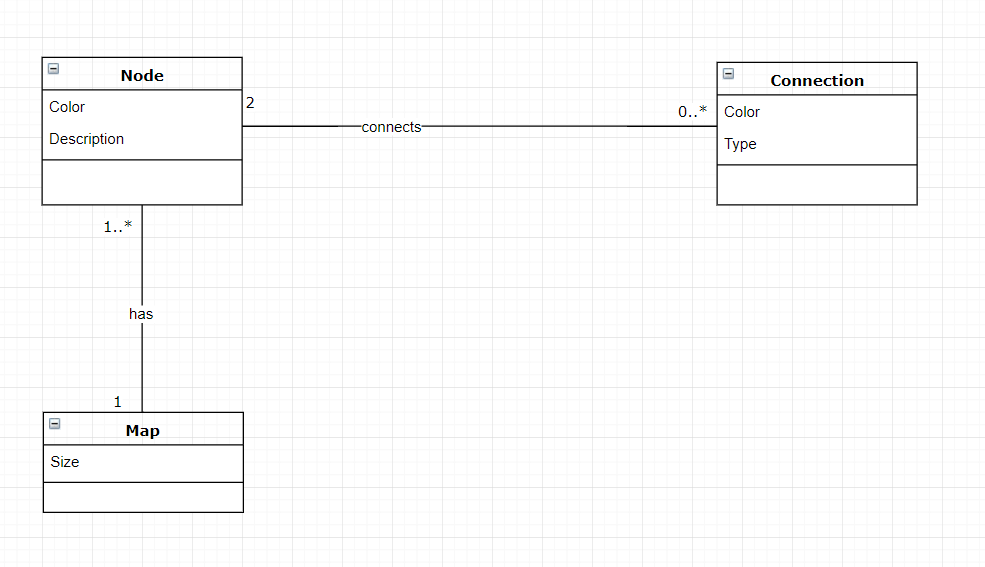
\includegraphics[scale=0.7]{images/DomainModel.png}
	\caption{Domainmodel}
	\label{fig:domain_model}
\end{figure}

Wie oben in der Grafik zu sehen ist, haben wir uns dafür entschieden, dass eine Map mindestens einen Knoten haben muss um eine Map zu sein. Im Moment denken wir das die Connection und die Map keine direkte Verbindung benötigen dies könnte sich aber beim Implementieren vielleicht noch ändern. Ebenfalls haben wird definiert, dass eine Verbindung immer zwischen 2 Knoten besteht.

\subsection{Assoziationen}
\label{subsec:assoziationen}
\begin{itemize}
\item Zwei Knoten haben keine oder mehrere Verbindungen. Eine Verbindung besteht aus 2 Knoten.
\item Eine Map hat einen oder Mehrere Knoten. Ein Knoten gehört zu einer Map.
\end{itemize}

\section{Use Cases}
\label{sec:use_cases}
Use-Cases beschreiben die Requirements der einzelnen Akteure, es zeigt die Abläufe des Programmes auf. Zeigt dabei aber nicht wie die einzelnen Teile funktionieren.

\subsection{Use Case Diagramm}
\label{subsec:use_case_diagramm}

\begin{figure}[H]
	\centering
		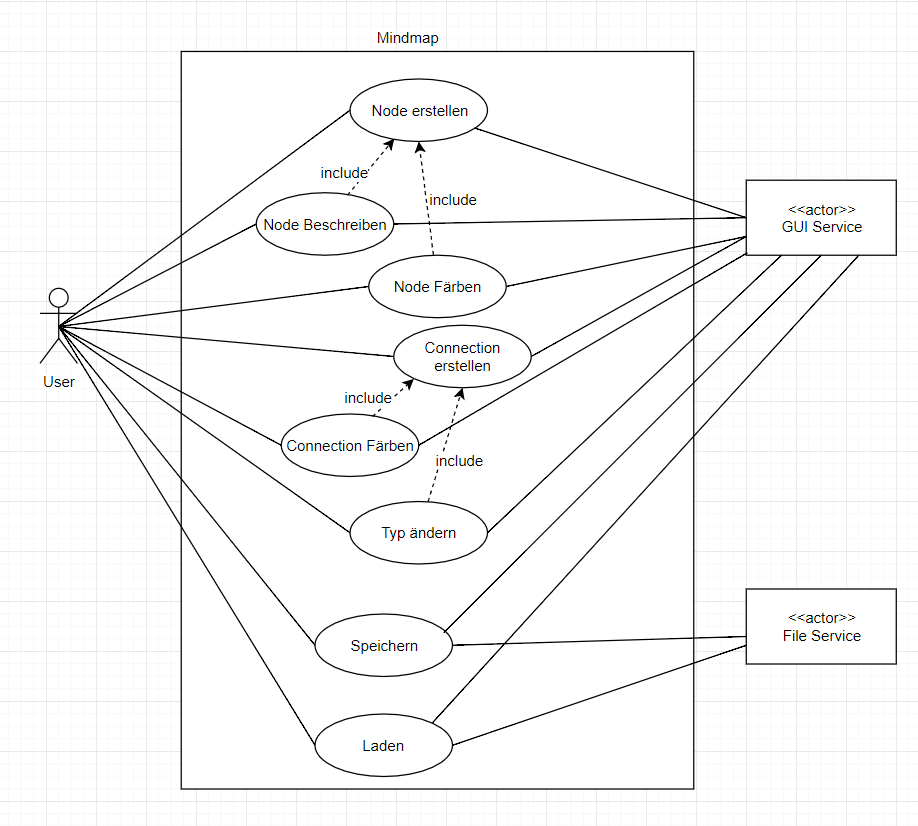
\includegraphics[scale=0.7]{images/UseCaseDiagram.PNG}
	\caption{Use Case Diagramm}
	\label{fig:use_case_diagramm}
\end{figure}

\subsection{Mindmap Process}
\label{subsec:mindmap_process}
Neues Mindmap Szenario:
\begin{enumerate}
\item Benutzer erstellt neues Mindmap
\item GUI Service zeigt leeres Mindmap an
\item Benutzer erstellt Nodes und Connections 
\item Benutzer bearbeitet die Nodes und Connections z.B. Typ, Beschreibung, Farbe.
\item GUI Service stellt dies dar
\item Punkt 3-5 werden wiederholt bis der Benutzer zufrieden ist
\item Benutzer speichert seine Arbeit
\item GUI Service übergibt Fileservice die Map
\item Fileservice speichert die Map in ein Dokument
\end{enumerate}

Mindmap bearbeiten Szenario: 
\begin{enumerate}
\item Benutzer lädt Mindmap
\item Fileservice lädt das alte Mindmap
\item GUI Service zeigt das Mindmap an (Danach analog zu oberem Szenario)
\end{enumerate}

\section{User Stories}
\label{sec:user_stories}
Eine User-Story beschreibt in ein oder zwei Sätzen eine gewünschte Funktion des Programmes.
\begin{enumerate}
\item Als Benutzer möchte ich, dass das Programm selbsterklärend und einfach zu bedienen ist.
\item Als Benutzer möchte ich ein Programm welches schnell startet und sich nicht langsam anfühlt.
\item Als Benutzer möchte ich ein optisch Ansprechendes Design. Als Benutzer finde ich ein Programm
besser wenn sein Design State of the Art ist.
\item Als Benutzer möchte ich, dass das Mindmap auf dem Papier gleich aussieht wie es im Programm ausgesehen hat.
\item Als Benutzer möchte ich nicht einen Experten konsultieren müssen um ein so triviales Programm zu installieren. 
\item Als Benutzer möchte ich mit dem Programm neue Mindmaps erstellen können.
\item Als Benutzer möchte ich neue Knoten hinzufügen können, welcher eine Beschreibung besitzt und wenn gewünscht auch eine spezielle Farbe haben kann. 
\item Als Benutzer möchte ich die verschiedenen Informationen, also Knoten miteinander vernetzen und so gruppieren können. 
\item Als Benutzer möchte ich meine Arbeit speichern können und gespeicherte Projekte auch wieder laden können
\item Als Benutzer möchte ich die Beschreibung eines Knoten auch nach seiner Erstellung bearbeiten können.
\item Als Benutzer möchte ich die Farbe eines Knotens nach seiner Erstellung bearbeiten können.
\item Als Benutzer möchte ich verschiedene Verbindungstypen definieren können, ich möchte Verbindungen zwischen verschiedenen Themen speziell hervorheben können. 
\item Als Benutzer möchte ich mein Mindmap drucken können.
\item Als Benutzer möchte ich mein Mindmap exportieren können, um es zum Beispiel als Bilddatei in einem Worddokument einfügen zu können.
\item Als Benutzer möchte ich ein Mindmap mit möglichst wenigen überschneidenden Verbindungen, das Programm sollte eine Möglichkeit bieten dieses Problem zu lösen.
\end{enumerate}

\section{Systemkontext}
\label{sec:systemkontext}
Der Systemkontext ist eine Beschreibung des Systems, seiner Teile und äusserlichen Einwirkungen auf das System.

Der Benutzer kann mit unserer Software ein Mindmap erstellen. Dies geschieht über eine grafische Benutzeroberfläche. Mit Hilfe eines Algorithmus können die Themen und Verbindungen des Mindmap optimal verteilt werden. Die Benutzeroberfläche und der Algorithmus sind Teil der Software\\
Die Software greift auf das Dateisystem des Computers zu um ein Mindmap zu speichern oder zu laden. Der Druckservice des Computers erlaubt das Drucken des Mindmaps. Diese beiden Teile liegen ausserhalb unserer Software.

\begin{figure}[H]
	\centering
		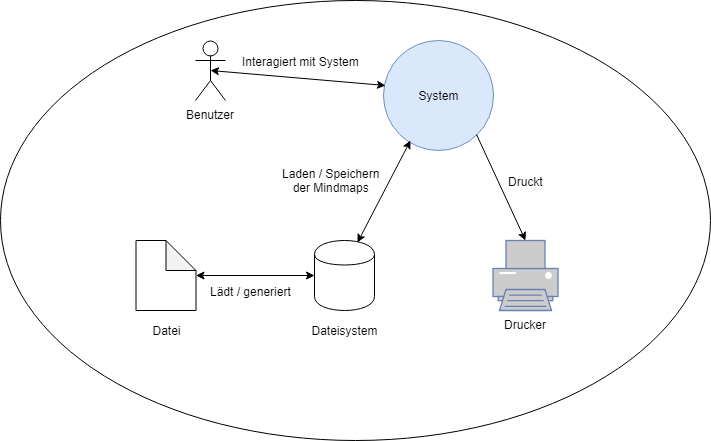
\includegraphics[scale=0.7]{images/Systemkontext.png}
	\caption{Systemkontext}
	\label{fig:systemkontext}
\end{figure}

\section{Anforderungen}
\label{sec:anforderungen}
--> Teil Modul Requirements Engineering

\chapter{Design}
\label{chap:design}

\section{System Sequence Diagram}
\label{sec:system_sequence_diagramm}
Die System Sequence Diagramme zeigen die möglichen Interaktionen 
von extern mit unserem Mindmap Programm.

\begin{figure}[H]
	\centering
		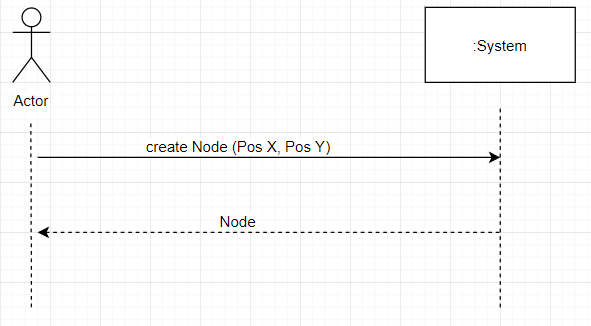
\includegraphics[scale=0.7]{images/createnode.PNG}
	\caption{Create Node SSD}
	\label{fig:create_node_ssd}
\end{figure}

Der Benutzer übergibt dem System eine Position in welcher er den Node erstellen möchte, das System
erstellt dann den Node mit allen seinen Komponenten, also der Form, dem Text und den Anchors für das
Verbinden.

\begin{figure}[H]
	\centering
		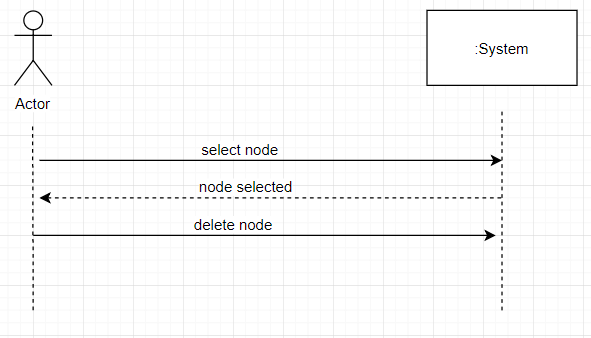
\includegraphics[scale=0.7]{images/deletenode.PNG}
	\caption{Delete Node SSD}
	\label{fig:delete_node_ssd}
\end{figure}
Der Benutzer wählt einen Node oder eine Verbindung(der Ablauf zum Löschen einens Nodes oder einer Verbindung ist gleich), das System löscht diesen Node dann vom GUI und von der Liste. 

\begin{figure}[H]
	\centering
		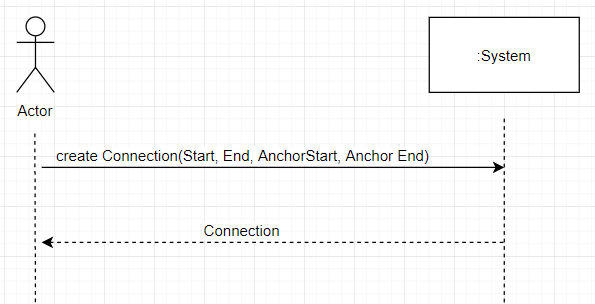
\includegraphics[scale=0.7]{images/createconnection.PNG}
	\caption{Create Connection SSD}
	\label{fig:create_connection_ssd}
\end{figure}
Der Benutzer wählt einen Start und einen Ziel Anchor für seine Verbindung aus, das System erstellt
dann anhand dieser Informationen die Verbindung.

\begin{figure}[H]
	\centering
		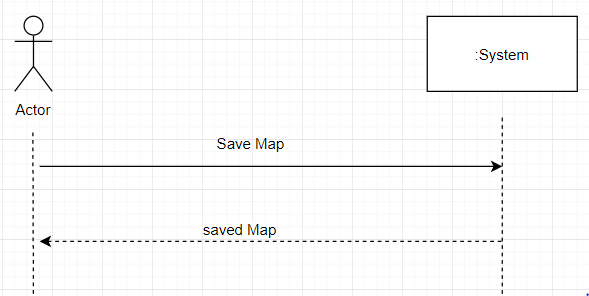
\includegraphics[scale=0.7]{images/savemap.PNG}
	\caption{Save Map SSD}
	\label{fig:save_map_ssd}
\end{figure}
Der Benuzer speichert die Map, das System speichert nun alle Informationen der Map in eine
Datei und übergibt sie dem Benutzer.

\begin{figure}[H]
	\centering
		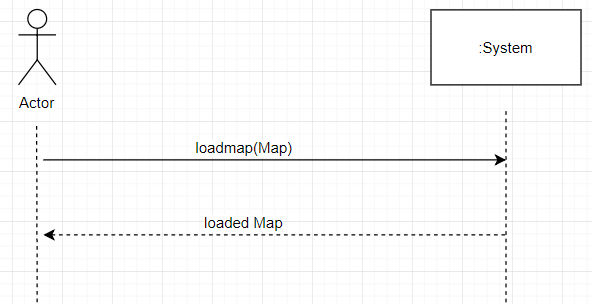
\includegraphics[scale=0.7]{images/loadmap.PNG}
	\caption{Load Map SSD}
	\label{fig:load_map_ssd}
\end{figure}
Der Benutzer lädt eine alte Map und übergibt dem System eine Datei mit den Informationen, das System
arbeitet nun die Informationen ab und stellt die Map dar.

\section{Sequence Diagram}
\label{sec:sequence_diagram}
Das Sequence Diagramm zeigt die Interaktion zwischen den verschiedenen Objekten in dem Mind Map System.
\begin{figure}[H]
	\centering
		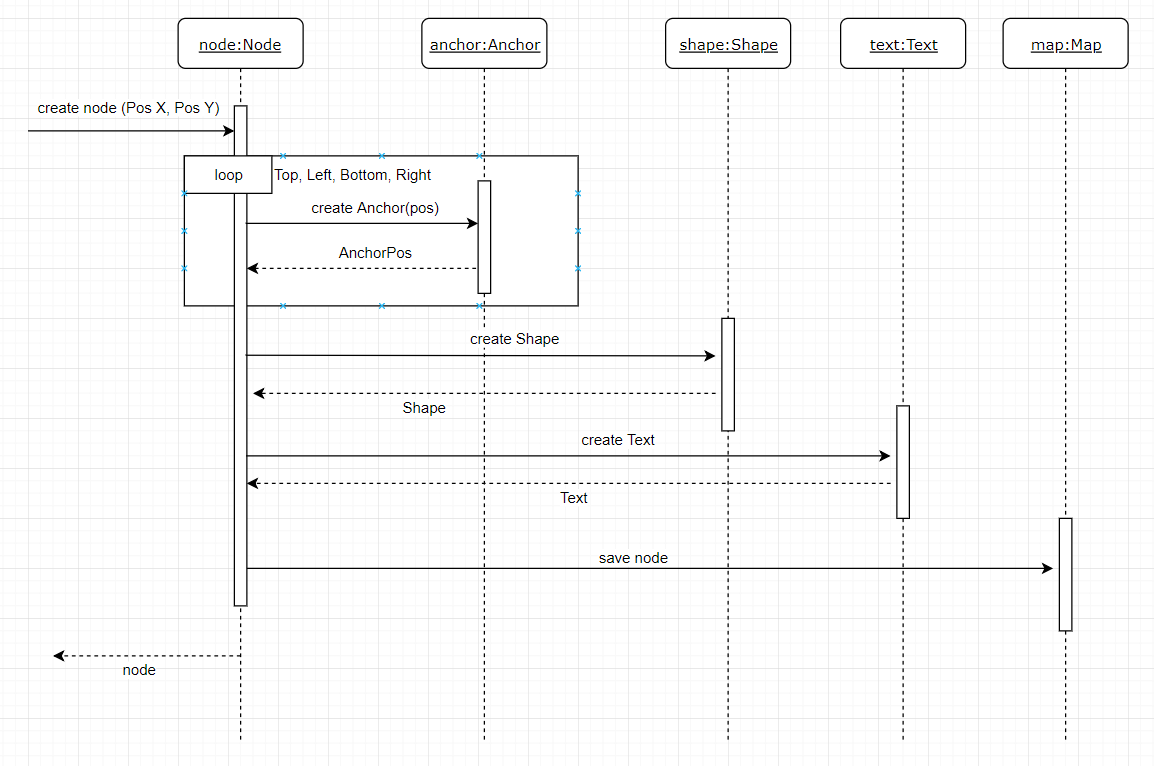
\includegraphics[scale=0.6]{images/crNodeSD.PNG}
	\caption{Create Node SD}
	\label{fig:create_node_SD}
\end{figure}

Das System erstellt einen neuen Node, der Node erstellt dann seine Objekte welche er benötigt.
Er erstellt ein Shape für seine Form, er erstellt einen Text für die Beschreibung und er erstellt
4 Anchors(TOP,LEFT,BOTTOM,RIGHT) für das Verbinden der Knoten. Danach wird der Knoten in die Maplist 
gespeichert.

\begin{figure}[H]
	\centering
		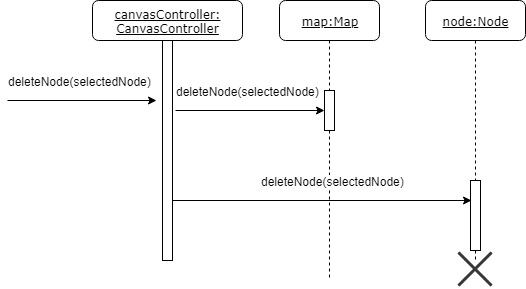
\includegraphics[scale=0.6]{images/delNodeSD.PNG}
	\caption{Delete Node SD}
	\label{fig:delete_node_SD}
\end{figure}

Das System löscht den selektieren Knoten von der Map und löscht diesen dann von der Liste. 
Dies funktioniert gleich bei der Verbindung.

\begin{figure}[H]
	\centering
		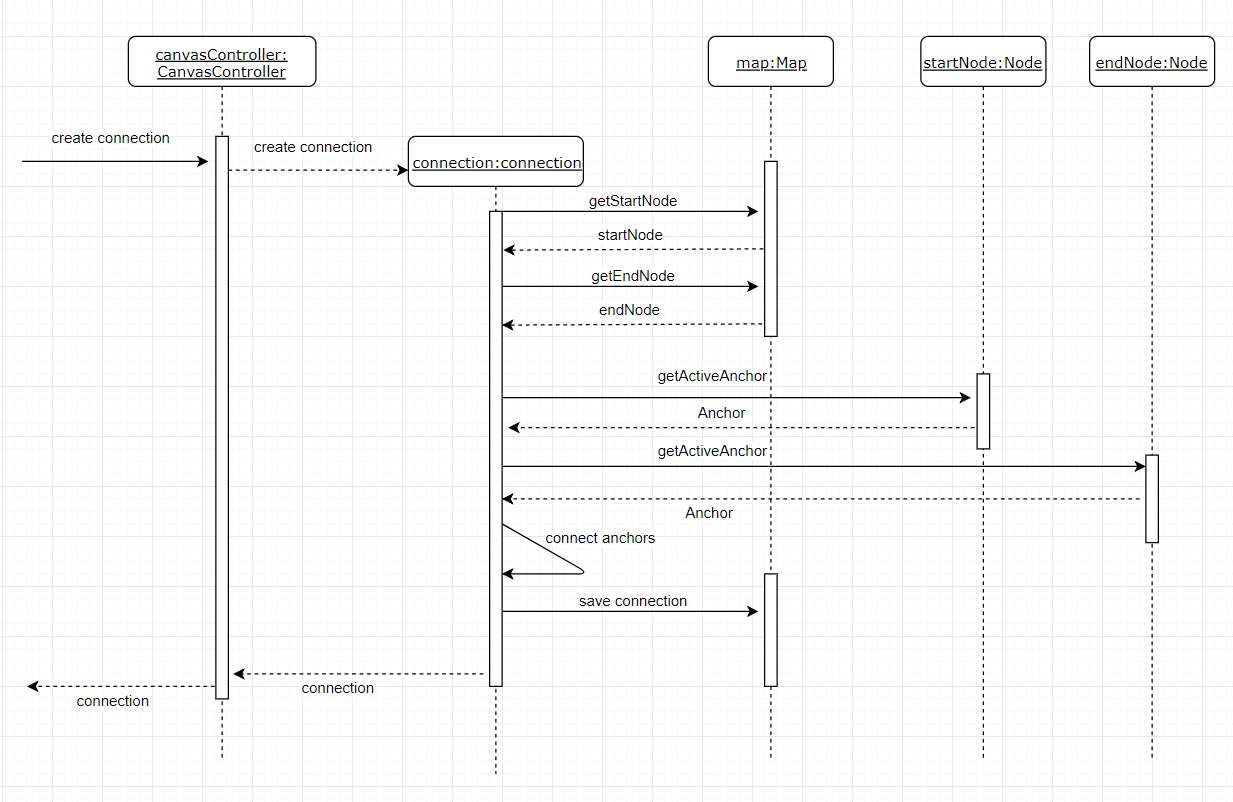
\includegraphics[scale=0.6]{images/connectionSD.PNG}
	\caption{Create Connection SD}
	\label{fig:create_connection_SD}
\end{figure}
Das System erstellt eine neue Verbindung, es holt sich zuerst die beiden aktiven Knoten, den Start 
und den End Knoten. Von diesen beiden Knoten holt es sich dann die jewiligen aktiven Anchors. Danach
verbindet das System die beiden aktiven Anchors miteinander.

\begin{figure}[H]
	\centering
		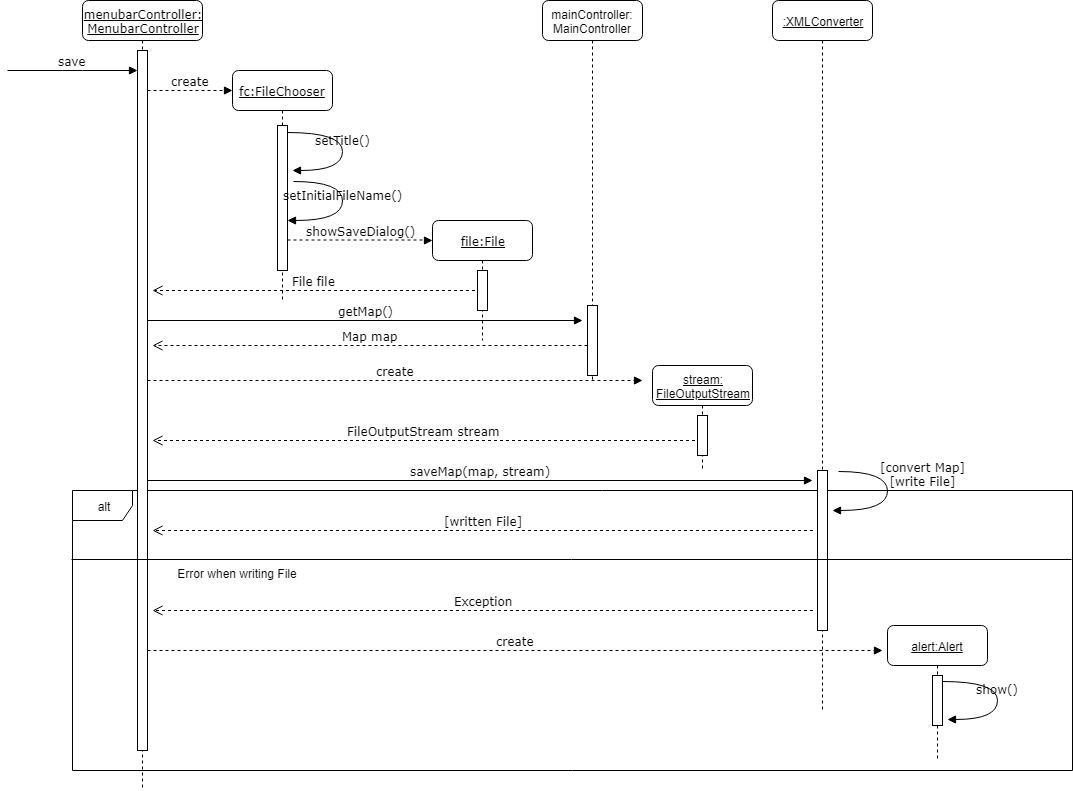
\includegraphics[scale=0.4]{images/savemapSD.png}
	\caption{Save Map SD}
	\label{fig:savemap_SD}
\end{figure}
Das System lässt den Benutzer eine Datei wählen und erzeugt einen OutputStream. Die Map des MainControllers und der Stream werden dem XMLConverter übergeben. Dieser konvertiert die Map in ein speicherbares Objekt und schreibt die XML Datei. Die Funktionalität des XMLConverters ist im nächsten Sequence Diagram ersichtlich.

\begin{figure}[H]
	\centering
		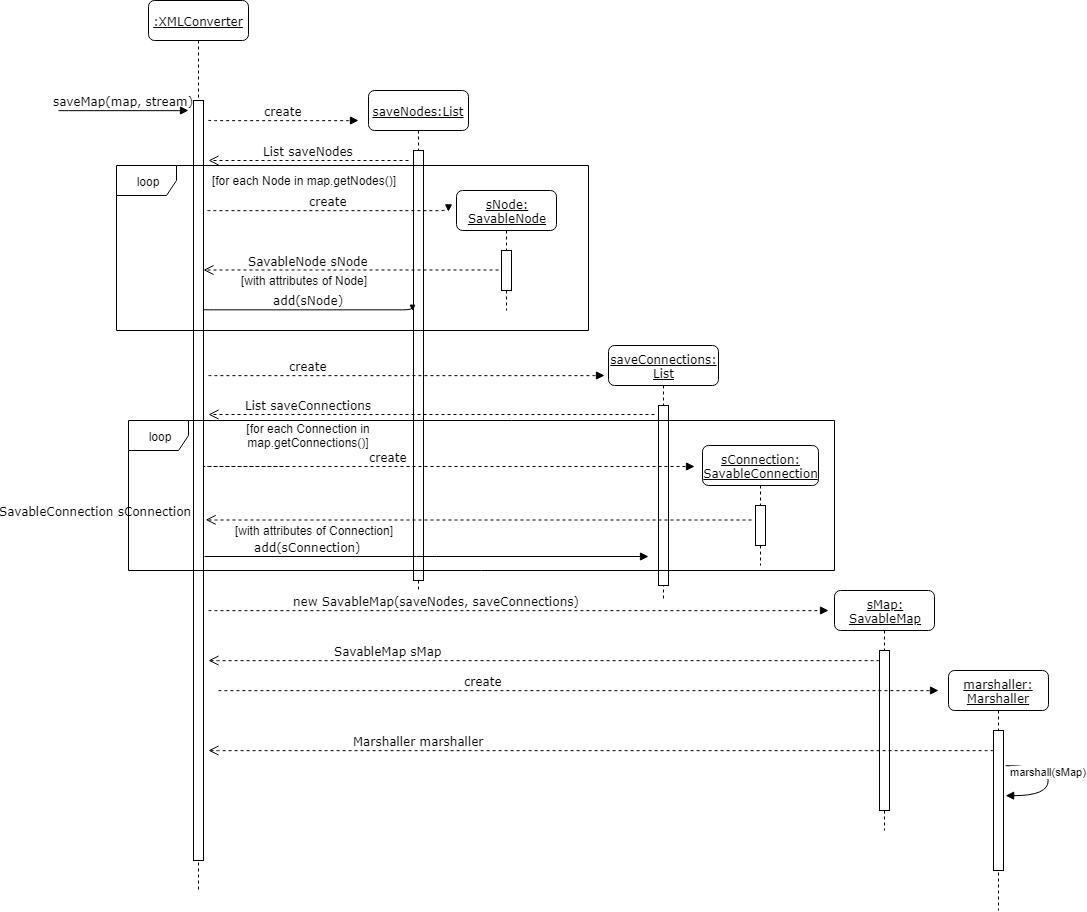
\includegraphics[scale=0.5]{images/saveConvertSD.png}
	\caption{Convert \& Save Map SD}
	\label{fig:saveConvert_SD}
\end{figure}

\begin{figure}[H]
	\centering
		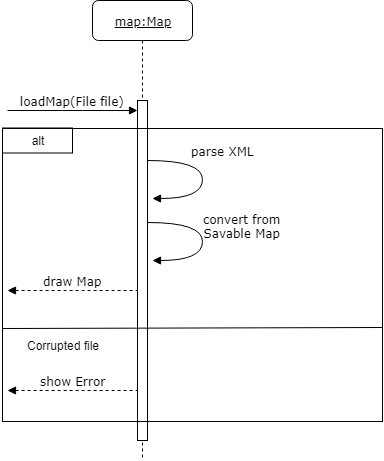
\includegraphics[scale=0.4]{images/loadmapSD.png}
	\caption{Load Map SD}
	\label{fig:loadmap_SD}
\end{figure}
Das System lässt den Benutzer eine Datei wählen. Der XMLConverter liest die Datei und erzeugt daraus eine Map. Diese wird danach angezeigt.

\begin{figure}[H]
	\centering
		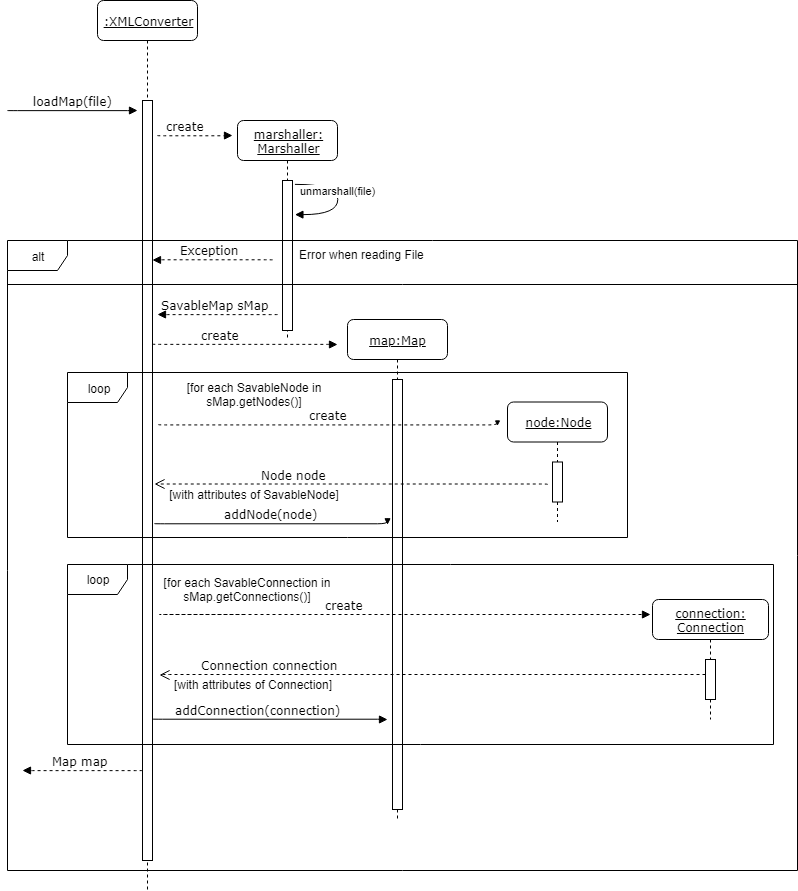
\includegraphics[scale=0.6]{images/loadConvertSD.png}
	\caption{Load \& Convert Map SD}
	\label{fig:loadConvert_SD}
\end{figure}

\section{Package Diagramm}
\label{sec:package_diagramm}
Unsere Packetstruktur ist nach dem MVC Prinzip erstellt. Wir haben ein View Packet mit den FXML Dateien und dem Main Programm, ein Controller Packet mit den Controllern, ein Util Packet mit den Zusatzfunktionen wie Speichern, Laden und Ordnen und ein Model Packet mit den Objekten wie Node, Connection usw.

\begin{figure}[H]
	\centering
		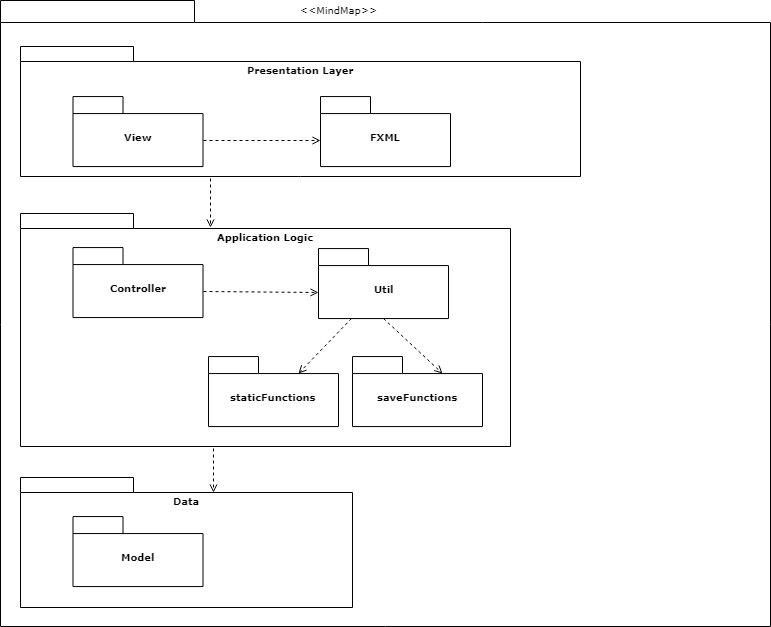
\includegraphics[scale=0.6]{images/packagediagramm.png}
	\caption{Package Diagramm}
	\label{fig:loadConvert_SD}
\end{figure}


\section{UML Diagramme}
\label{sec:uml_diagramme}
\chapter{Entwicklung}
\label{chap:entwicklung}
In diesem Kapitel wird die Vorgehensweise und die Realisierung der Entwicklung dokumentiert.
\section{Sprint Planung}
\label{sec:sprintplanung}
Wir haben uns entschieden das Projekt in Sprints zu unterteilen. Diese Art der Planung erschien uns am praktischsten, da wir so einen guten Überblick hatten wann was fällig ist. Die Sprintplanung wurde im Gitlab integrierten Board gemacht. Zu jeder Userstory wurde ein Issue erstellt und auf die jeweiligen Sprints verteilt.
\begin{figure}[H]
	\centering
		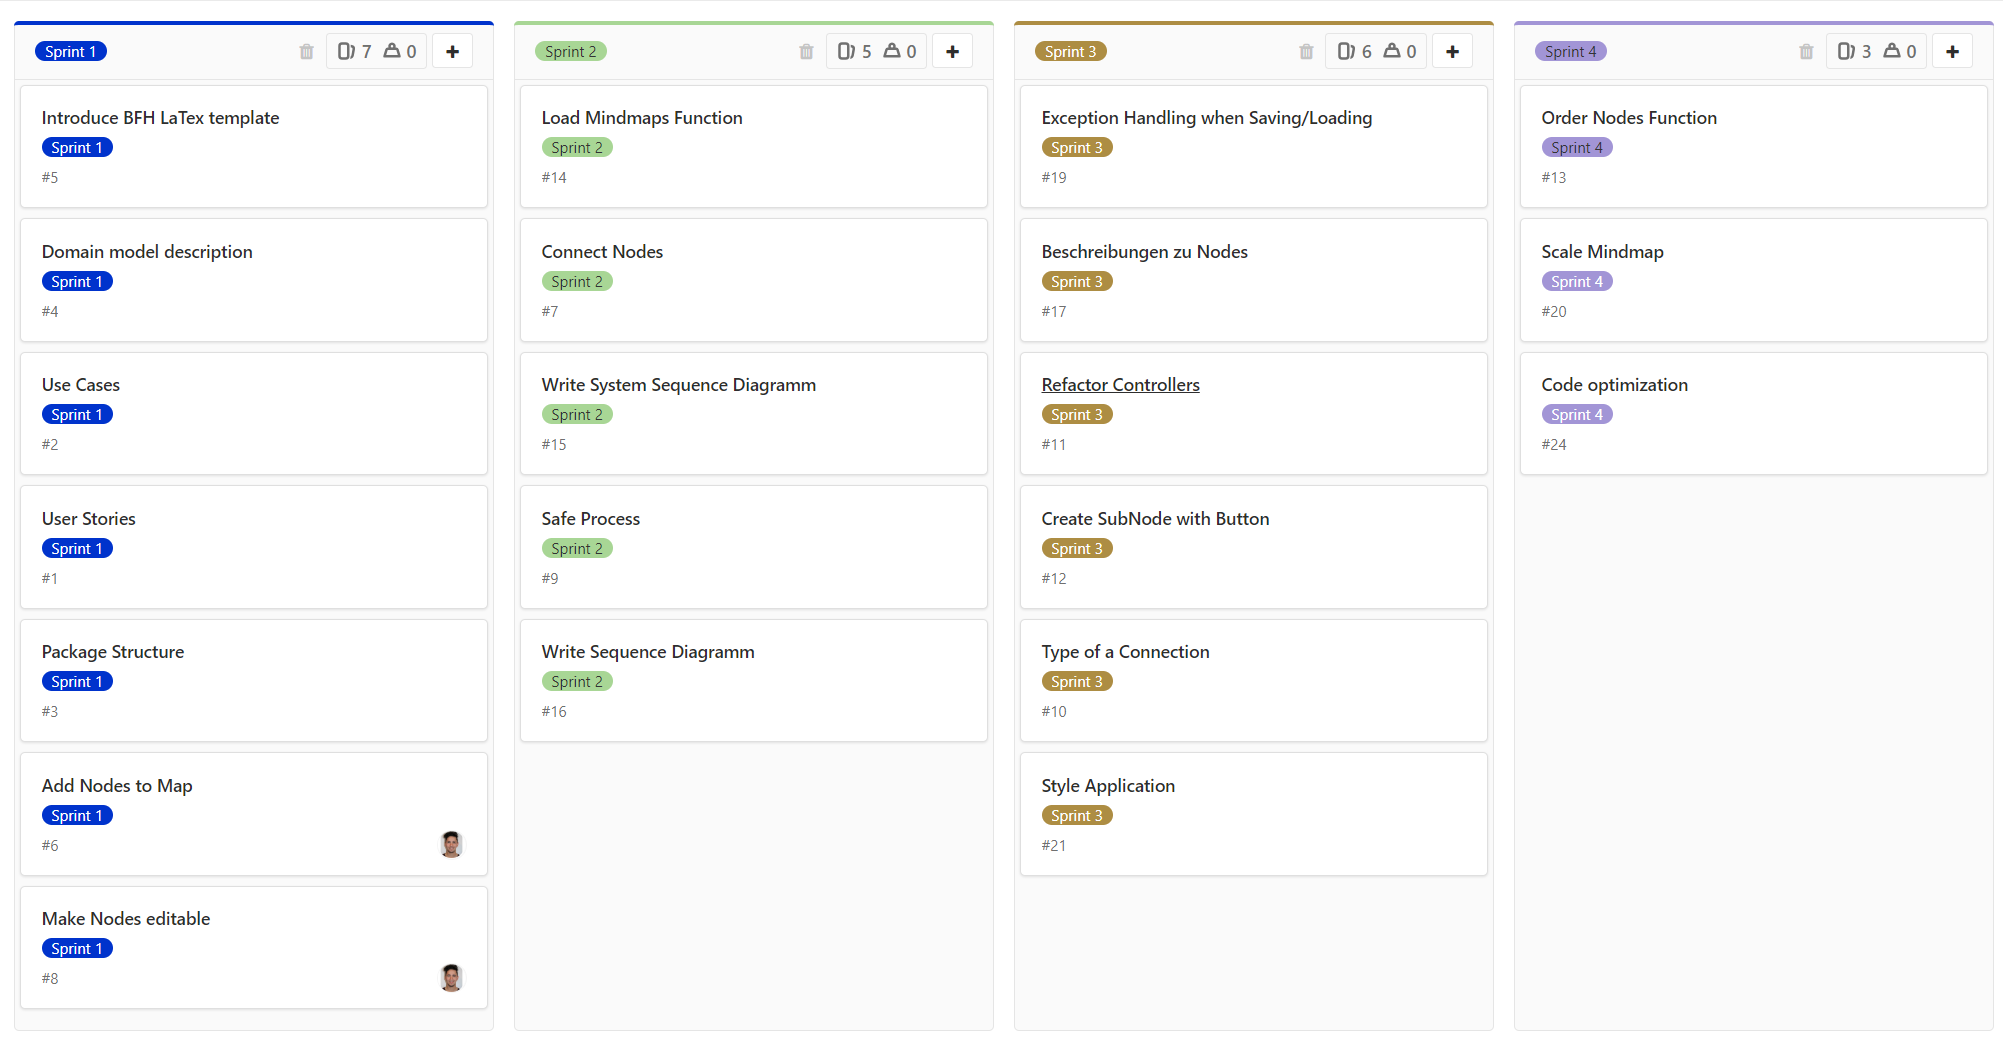
\includegraphics[width=\textwidth]{images/Board.PNG}
	\caption{Sprint Plannung}
	\label{fig:sprint_plannung}
\end{figure}

\section{Sprint 1}
\label{sec:sprint_1}
Der Sprint 1 dauerte vom 13.03 - 03.04. In diesem Sprint haben wir primär den Fokus auf die Dokumentation und die Planung gelegt. Ebenfalls haben wir uns entschieden eine Desktop Applikation zu schreiben mit JavaFX. Zusätzlich wurde ein kleiner Prototyp des Programmes erstellt. Erste Funktionen wie das Erstellen von Knoten und deren Verschiebung wurde ebenfalls realisiert.
\section{Sprint 2}
\label{sec:sprint_2}
Der Sprint 2 dauerte vom 03.04 - 24.04. In diesem Sprint wurde dann richtig begonnen mit dem Programmieren der Funktionalitäten. Es wurden ebenfalls die SD/SSD Diagramme erstellt. Realisiert wurden die Funktionen zum Verbinden von Knoten und das Laden und Speichern der Knoten. Zum Laden und Speichern der Knoten haben wir uns für JAXB for Java entschieden. Dieses Framework erlaubt es aus Objekten XML Dateien zu erstellen.
In diesem Sprint haben wir bemerkt, dass unser Programm zu unübersichtlich wird, wir haben unsere Kontrollerstruktur daraufhin angepasst.
\section{Sprint 3}
\label{sec:sprint_3}
Der Sprint 3 dauert vom 24.04 - 15.05. In diesem Sprint wurde vor allem zuerst ein grosses Refactoring des Codes gemacht. Der Hauptkontroller wurde in 3 Unterkontroller geteilt. Dies gab dem Programm mehr Lesbarkeit und war infolgedessen auch einfacher zu erweitern. Ebenfalls wurde das Feature zur Zusatzinformation für Knoten, der Unterknoten Button und der Typ einer Verbindung hinzugefügt. Am Schluss des Sprints wurde dann noch die Applikation optisch verschönert.
\section{Sprint 4}
\label{sec:sprint_4}
Der Sprint 4 dauert vom 15.05 - 29.05. In diesem Sprint wurde das Programm beendet. Diverse Bugs wurden ausgebessert und einzelne neue Funktionen wie das Skalieren der Applikation und die ordnen Funktion wurde hinzugefügt. 

\section{Kontroller Management}
\label{sec:controller_mgmnt}
Das Programm besitzt 4 Kontroller, die jeweils einer FXML Datei zugeordnet sind. Der MainController ist dabei die Schnittstelle zwischen der View und den Kontrollern. Der CanvasController ist für alle Aktionen im Programmfeld zuständig, er erstellt zum Beispiel neue Knoten oder färbt diese. Der MenuBarController ist für die Aktionen in der Menubar zuständig, er speichert und lädt die Maps. Zuletzt noch der ToolbarController, dieser prüft primär welche Aktionen im CanvasController ausgeführt werden sollen, wie z.b. Knoten erstellen, Verbinden usw.

\section{Ordnungs Funktion}
\label{sec:controller_mgmnt}
Die Knoten Ordnen Funktion wurde implementiert um dem Benutzer zu helfen sein Mindmap aufzuräumen.
Die Funktion kann dabei 3 Probleme erkennen. 
\begin{figure}[H]
	\centering
		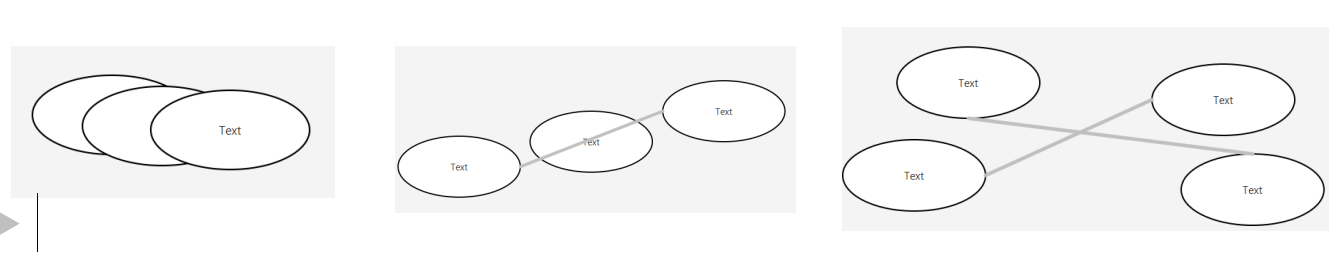
\includegraphics[width=\textwidth]{images/threeissues.PNG}
	\caption{3 erkennbare Probleme}
	\label{fig:probleme}
\end{figure}

Diese 3 Probleme versucht nun der Algorithmus zu lösen. Er geht dabei nach einem Try and Error konzept vor. Es wird versucht den Knoten in 8 Richtungen zu verschieben und geprüft ob das Problem gelöst wurde. Falls nicht, wird die Distanz bis auf 7x vergrössert. Die Distanz des Verschiebens ist jeweils der Radius der zu verschiebenden Ellipse. 

\begin{figure}[H]
	\centering
		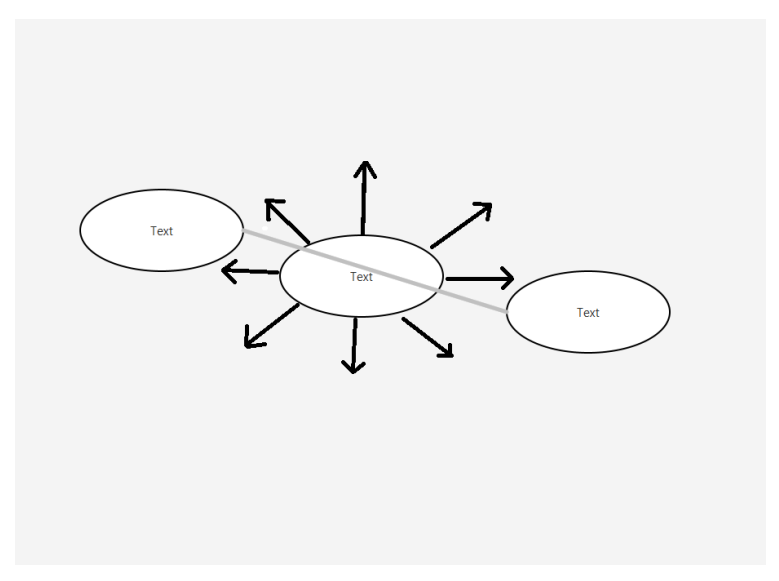
\includegraphics[scale=0.5]{images/solving.PNG}
	\caption{Problemlösung}
	\label{fig:problemloesung}
\end{figure}

\section{Testing}
\label{sec:testing}
Leider haben wir im Programm keine Tests implementiert, beim Programm wurde von Hand das Frontend getestet. Wir hatten grosse Probleme die Frontend Tests zu implementieren. Auch backendtests
liefen nicht da wir Probleme hatten die JavaFX Elemente einzubinden. Als Ausblick müssten diese 
auf jeden Fall noch implementiert werden.


Das Fazit zu dieser Lösung ist, dass der Algorithmus bei einfachen Problemen ohne Probleme eine Lösung findet. Bei schwereren Problemen jedoch findet er teils keine Lösung. Ebenfalls ist der Algorithmus sehr ineffizient und kann lange dauern wenn sehr viele Knoten geprüft werden müssen. 

\section{Programm ausführen}
\label{sec:run_program}

\subsection{Tools and Software}
\label{subsec:tools}
Unsere Mindmap Applikation benutzt folgende Software und Frameworks.
\begin{itemize}
\item Java jdk1.8.0\_{}191
\item JavaFX http://javafx.com/javafx/8.0.191
\item JavaFX Scene Builder 10.0.0
\end{itemize}

\subsection{Installation}
Um das Programm auszuführen muss zu erst das Repository per Git geklont werden.
\begin{verbatim}
git clone https://gitlab.ti.bfh.ch/rascl1/mindmap.git
\end{verbatim}
Wenn das Projekt in ein IDE importiert wird, muss der Ordner "{}MindMap"{} als Grundlage gewählt werden.\\
Oder das Programm kann mit der \texttt{MindMap.jar} ausgeführt werden.




\chapter{Fazit}
\label{chap:fazit}
Das Fazit dieses Projektes ist, dass wir sehr viel gelernt haben. Es war wichtig für uns nach dem Software Engineering Modul noch einmal ein Projekt durchzuführen. Wir liefen dabei in einige Schwierigkeiten, wir hätten zum Beispiel die Kontrollerstruktur von Anfang an erstellen müssen. Es war sehr mühsam die Struktur in der Mitte der Entwicklung zu ändern. Die Applikation an sich ist nicht schlecht und wir sind relativ zufrieden mit dem Ergebnis. Das Produkt hätte aber teilweise besser implementiert werden können, das Verbinden von Knoten hätte besser gelöst werden können, ebenfalls fühlt sich das Programm zum Teil steiff an. Das Fazit ist also, dass wir sehr viel gelernt haben und somit das Projekt ein Erfolg war.
%---------------------------------------------------------------------------

% Selbständigkeitserklärung
%---------------------------------------------------------------------------
%\cleardoublepage
%\phantomsection 
%\addcontentsline{toc}{chapter}{Selbständigkeitserklärung}
%\include{vorspann/selbstaendigkeitserklaerung}
%---------------------------------------------------------------------------

% Glossary
%---------------------------------------------------------------------------
%\cleardoublepage
%\phantomsection 
%\addcontentsline{toc}{chapter}{Glossar}
%\renewcommand{\glossaryname}{Glossar}
%\printglossary
%---------------------------------------------------------------------------

% Bibliography
%---------------------------------------------------------------------------
%\cleardoublepage
%\phantomsection 
%\addcontentsline{toc}{chapter}{Literaturverzeichnis}
%\bibliographystyle{IEEEtranS}
%\bibliography{data/bibliography}{}
%---------------------------------------------------------------------------

% Listings
%---------------------------------------------------------------------------
\cleardoublepage
\phantomsection 
\addcontentsline{toc}{chapter}{Abbildungsverzeichnis}
\listoffigures
%\cleardoublepage
%\phantomsection 
%\addcontentsline{toc}{chapter}{Tabellenverzeichnis}
%\listoftables
%---------------------------------------------------------------------------

% Index
%---------------------------------------------------------------------------
%\cleardoublepage
%\phantomsection 
%\addcontentsline{toc}{chapter}{Stichwortverzeichnis}
%\renewcommand{\indexname}{Stichwortverzeichnis}
%\printindex
%---------------------------------------------------------------------------

% Attachment:
%---------------------------------------------------------------------------
\appendix
\settocdepth{section}
\chapter{Use Cases}
\label{chap:use_cases}

\section*{Use Case 1: Knoten erstellen}
\begin{itemize}
\item \textbf{Titel:} Als Benutzer möchte ich einen Knoten erstellen können.
\item \textbf{Voraussetzung:} Programm ist gestartet
\item \textbf{Erfolgsszenario:}
	\begin{enumerate}
	\item Der Benutzer gibt den Befehl einen neuen Knoten zu erstellen.
	\item Das Programm fügt den neuen Knoten dem Mindmap hinzu.
	\end{enumerate}
\item \textbf{Nachbedingung:} Ein neuer Knoten wurde dem Mindmap hinzugefügt.
\item \textbf{Alternative Szenarien:}
	\begin{enumerate}
	\item [1.a 1] Der Benutzer schreibt eine Beschreibung für den Knoten.
	\item []
	\item [1.b 1] Der Benutzer ändert die Farbe des Knoten.
	\end{enumerate}
\end{itemize}

\section*{Use Case 2: Knoten verbinden}
\begin{itemize}
\item \textbf{Titel:} Als Benutzer möchte ich zwei Knoten miteinander verbinden können.
\item \textbf{Voraussetzung:} Ein Mindmap mit mindestens zwei Knoten wurde erstellt oder geladen.
\item \textbf{Erfolgsszenario:}
	\begin{enumerate}
	\item Der Benutzer wählt zwei Knoten aus.
	\item Das Programm verbindet die ausgewählten Knoten.
	\end{enumerate}
\item \textbf{Nachbedingung:} Zwischen den ausgewählten Knoten besteht eine Verbindung.
\item \textbf{Alternative Szenarien:}
	\begin{enumerate}
	\item [1.a 1] Der Benutzer ändert die Art der Verbindung.
	\end{enumerate}
\end{itemize}

\section*{Use Case 3: Mindmap speichern}
\begin{itemize}
\item \textbf{Titel:} Als Benutzer möchte ich ein Mindmap speichern können.
\item \textbf{Voraussetzung:} Ein Mindmap wurde erstellt.
\item \textbf{Erfolgsszenario:}
	\begin{enumerate}
	\item Der Benutzer wählt einen Speicherort.
	\item Das Programm übergibt dem Filesystem eine Datei.
	\end{enumerate}
\item \textbf{Nachbedingung:} Eine Datei mit den Informationen des Mindmaps wurde am gewählten Ort im Filesystem gespeichert.
\item \textbf{Alternative Szenarien:}
	\begin{enumerate}
	\item [2.a 1] Das Filesystem verweigert das Speichern wegen zu wenig Speicherplatz.
	\item [2.a 2] Das Programm informiert den Benutzer, dass nicht genug Speicherplatz vorhanden ist.
	\item []
	\item [2.b 1] Das Filesystem verweigert den Zugriff auf den Speicherort.
	\item [2.b 2] Das Programm informiert den Benutzer, dass der Zugriff verweigert wurde.
	\end{enumerate}
\end{itemize}

\section*{Use Case 4: Mindmap laden}
\begin{itemize}
\item \textbf{Titel:} Als Benutzer möchte ich ein gespeichertes Mindmap laden können.
\item \textbf{Voraussetzung:} Eine Datei mit den Informationen eines Mindmap existiert im Filesystem.
\item \textbf{Erfolgsszenario:}
	\begin{enumerate}
	\item Der Benutzer wählt eine Datei aus.
	\item Das Programm lädt die Datei.
	\item Das Programm zeigt das geladene Mindmap an.
	\end{enumerate}
\item \textbf{Nachbedingung:} Das Programm zeigt ein Mindmap mit den Informationen aus der geladenen Datei.
\item \textbf{Alternative Szenarien:}
	\begin{enumerate}
	\item [2.a 1] Das Filesystem verweigert den Zugriff auf die Datei.
	\item [2.a 2] Das Programm informiert den Benutzer, dass der Zugriff verweigert wurde.
	\item []
	\item [2.b 1] Das Programm lädt eine beschädigte Datei.
	\item [2.b 2] Das Programm informiert den Benutzer, dass die Datei beschädigt ist und nicht geladen werden kann.
	\end{enumerate}
\end{itemize}

\section*{Use Case 5: Knoten verändern}
\begin{itemize}
\item \textbf{Titel:} Als Benutzer möchte ich einen erstellten Knoten verändern können.
\item \textbf{Voraussetzung:} Ein Mindmap mit mindestens einem Knoten wurde erstellt oder geladen.
\item \textbf{Erfolgsszenario:}
	\begin{enumerate}
	\item Der Benutzer wählt einen existierenden Knoten.
	\item Der Benutzer schreibt eine (neue) Beschreibung für den Knoten.
	\end{enumerate}
\item \textbf{Nachbedingung:} Der gewählte Knoten wurde verändert.
\item \textbf{Alternative Szenarien:}
	\begin{enumerate}
	\item [2.a 1] Der Benutzer wählt eine (neue) Farbe für den Knoten.
	\end{enumerate}
\end{itemize}

\section*{Use Case 6: Verbindung verändern}
\begin{itemize}
\item \textbf{Titel:} Als Benutzer möchte ich verschiedene Verbindungstypen definieren können.
\item \textbf{Voraussetzung:} Ein Mindmap mit mindestens zwei Knoten wurde erstellt oder geladen.
\item \textbf{Erfolgsszenario:}
	\begin{enumerate}
	\item Der Benutzer wählt eine Verbindung aus.
	\item Der Benutzer ändert die Art/die Darstellung der Verbindung.
	\end{enumerate}
\item \textbf{Nachbedingung:} Die gewählte Verbindung wurde verändert.
\end{itemize}

\section*{Use Case 7: Mindmap drucken}
\begin{itemize}
\item \textbf{Titel:} Als Benutzer möchte ich ein Mindmap drucken können.
\item \textbf{Voraussetzung:} Ein Mindmap wurde erstellt oder geladen.
\item \textbf{Erfolgsszenario:}
	\begin{enumerate}
	\item Der Benutzer gibt den Befehl das Mindmap zu drucken.
	\item Das Programm sendet eine Datei an den Drucker.
	\end{enumerate}
\item \textbf{Nachbedingung:} Das Mindmap wurde ausgedruckt.
\item \textbf{Alternative Szenarien:}
	\begin{enumerate}
	\item [2.a 1] Das Programm informiert den Benutzer, dass kein Drucker angeschlossen ist.
	\item []
	\item [2.b 1] Das Programm informiert den Benutzer, dass die gesendete Datei vom Drucker zurückgewiesen wurde.
	\end{enumerate}
\end{itemize}

\section*{Use Case 8: Mindmap exportieren}
\begin{itemize}
\item \textbf{Titel:} Als Benutzer möchte ich ein Mindmap exportieren können.
\item \textbf{Voraussetzung:} Ein Mindmap wurde erstellt oder geladen.
\item \textbf{Erfolgsszenario:}
	\begin{enumerate}
	\item Der Benutzer wählt ein Dateiformat.
	\item Der Benutzer wählt einen Speicherort.
	\item Das Programm übergibt dem Filesystem eine Datei mit dem gewünschten Format.
	\end{enumerate}
\item \textbf{Nachbedingung:}
\item \textbf{Alternative Szenarien:}
	\begin{enumerate}
	\item [2.a 1] Das Filesystem verweigert das Speichern wegen zu wenig Speicherplatz.
	\item [2.a 2] Das Programm informiert den Benutzer, dass nicht genug Speicherplatz vorhanden ist.
	\item []
	\item [2.b 1] Das Filesystem verweigert den Zugriff auf den Speicherort.
	\item [2.b 2] Das Programm informiert den Benutzer, dass der Zugriff verweigert wurde.
	\end{enumerate}
\end{itemize}

\section*{Use Case 9: Darstellung optimieren}
\begin{itemize}
\item \textbf{Titel:} Als Benutzer möchte ich die Darstellung des Mindmaps optimieren können.
\item \textbf{Voraussetzung:} Ein Mindmap wurde erstellt oder geladen.
\item \textbf{Erfolgsszenario:}
	\begin{enumerate}
	\item Der Benutzer gibt den Befehl das Mindmap zu optimieren.
	\item Das Programm optimiert das Mindmap.
	\end{enumerate}
\item \textbf{Nachbedingung:} Ein Mindmap mit möglichst wenig sich überschneidenden Verbindungen.
\end{itemize}

%---------------------------------------------------------------------------

%---------------------------------------------------------------------------
\end{document}

